\chapter{L’île de Pâques}
\section*{8 mars 2015}
Petite entorse au règlement du voyage, je suis parti 3 jours sur l'île de Pâques sans le vélo. Il est resté à Santiago chez Nelson, un chilien qui m´a hébergé en Couchsurfing. \newline
 Camping au bord de l'océan dans la petite ville d'Hanga Roa, la seule de l'île. \newline
 \newline
\centerline{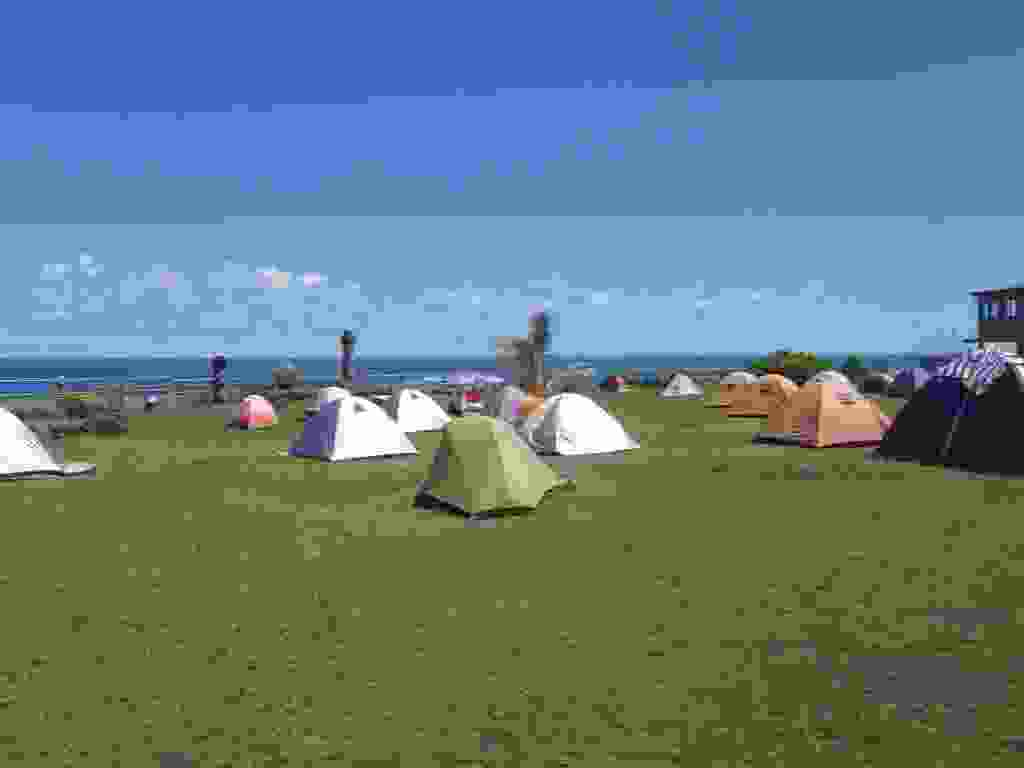
\includegraphics[width=\mywidth]{../wp-content/uploads/2015/03/P3012436-1024x768.jpg} } 
Petite balade au bord de l´eau et les premiers Moais sont là. \newline
 \newline
\centerline{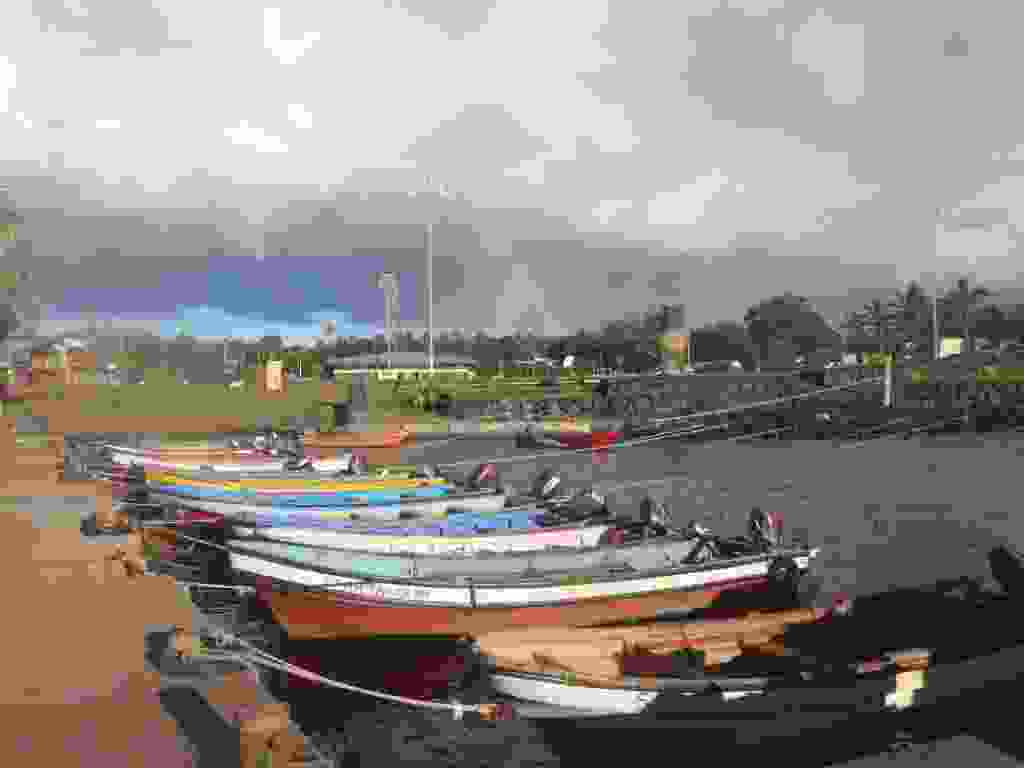
\includegraphics[width=\mywidth]{../wp-content/uploads/2015/03/P3032529-1024x768.jpg} } 
\newline
\centerline{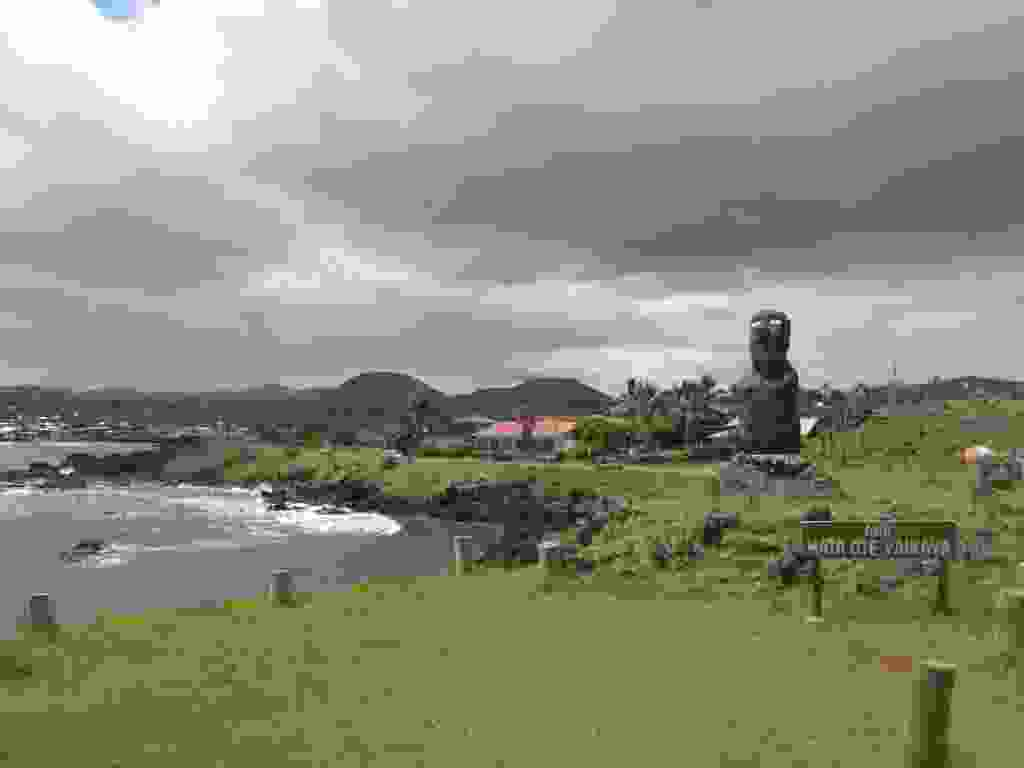
\includegraphics[width=\mywidth]{../wp-content/uploads/2015/03/P3012439-1024x768.jpg} } 
 \newline
\centerline{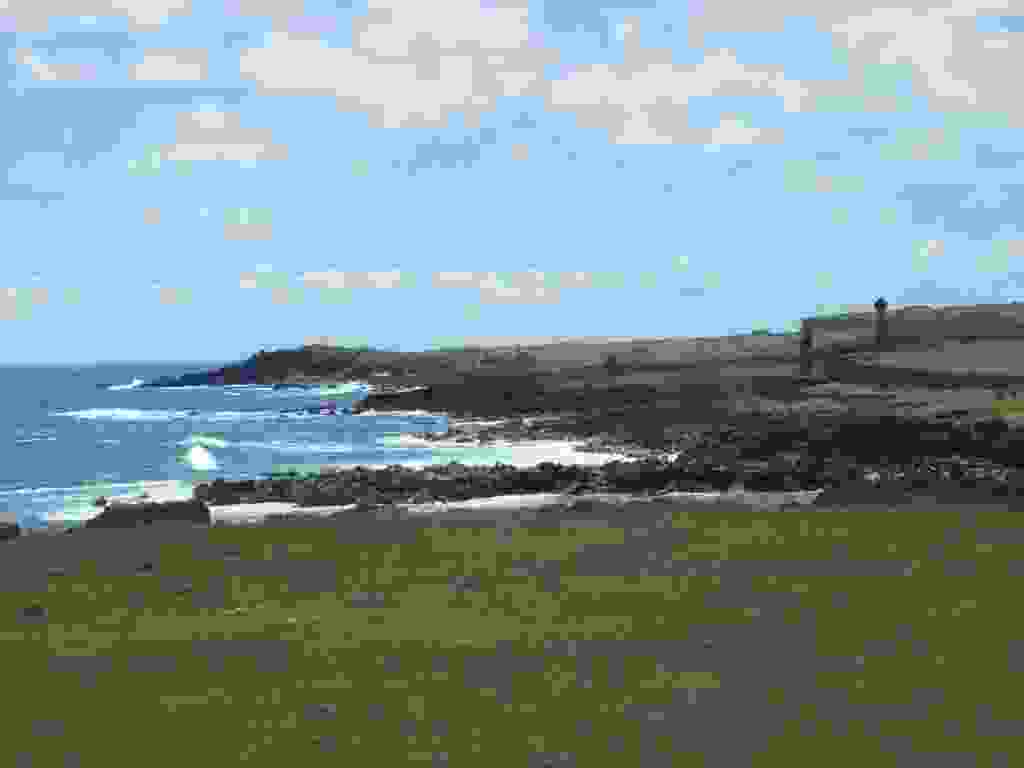
\includegraphics[width=\mywidth]{../wp-content/uploads/2015/03/P3012444-1024x768.jpg} } 
 \newline
\centerline{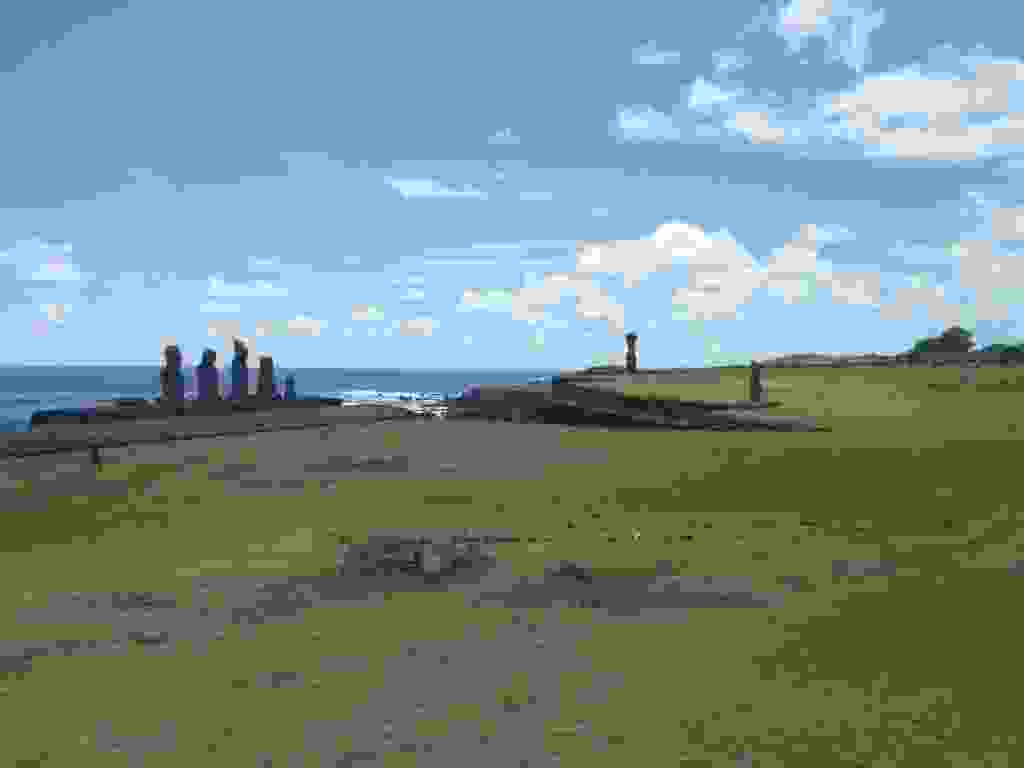
\includegraphics[width=\mywidth]{../wp-content/uploads/2015/03/P3012445-1024x768.jpg} } 
 \newline
\centerline{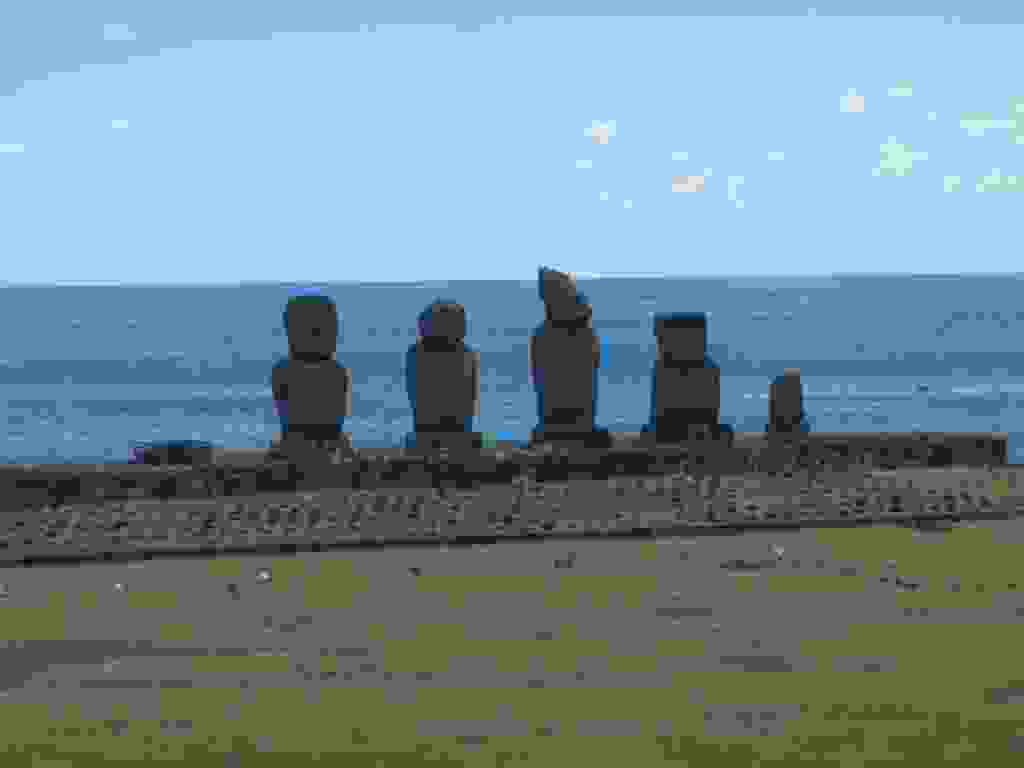
\includegraphics[width=\mywidth]{../wp-content/uploads/2015/03/P3012446-1024x768.jpg} } 
\newline
\centerline{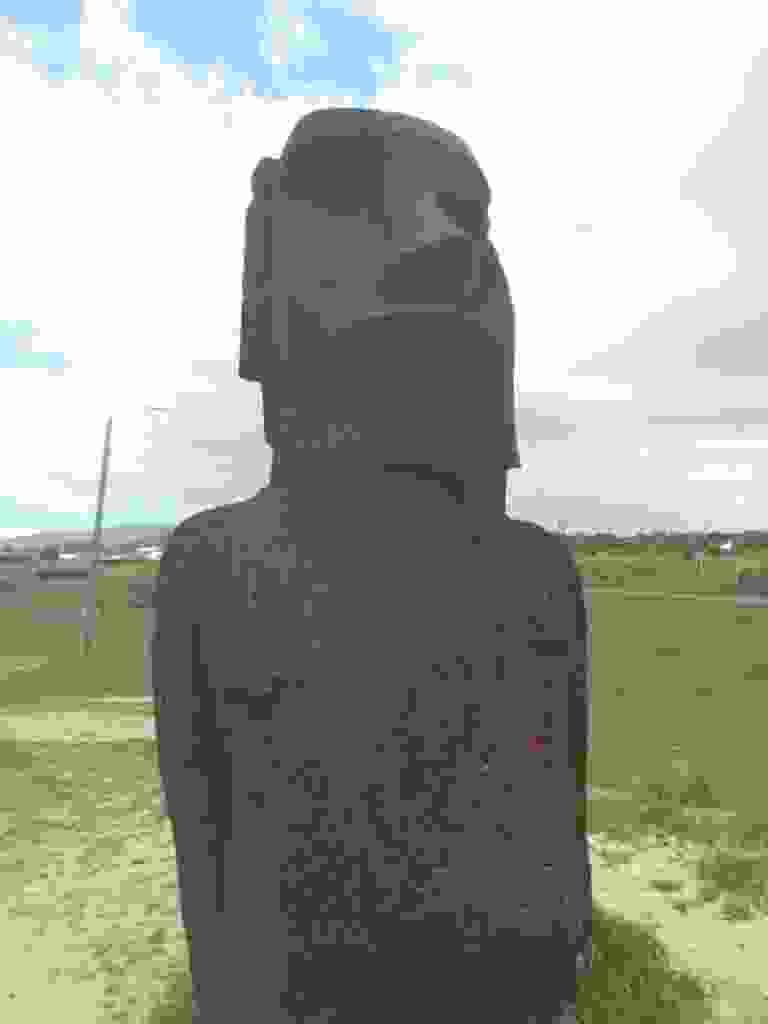
\includegraphics[width=\mywidth]{../wp-content/uploads/2015/03/P3012443-768x1024.jpg} } 
 \newline
\centerline{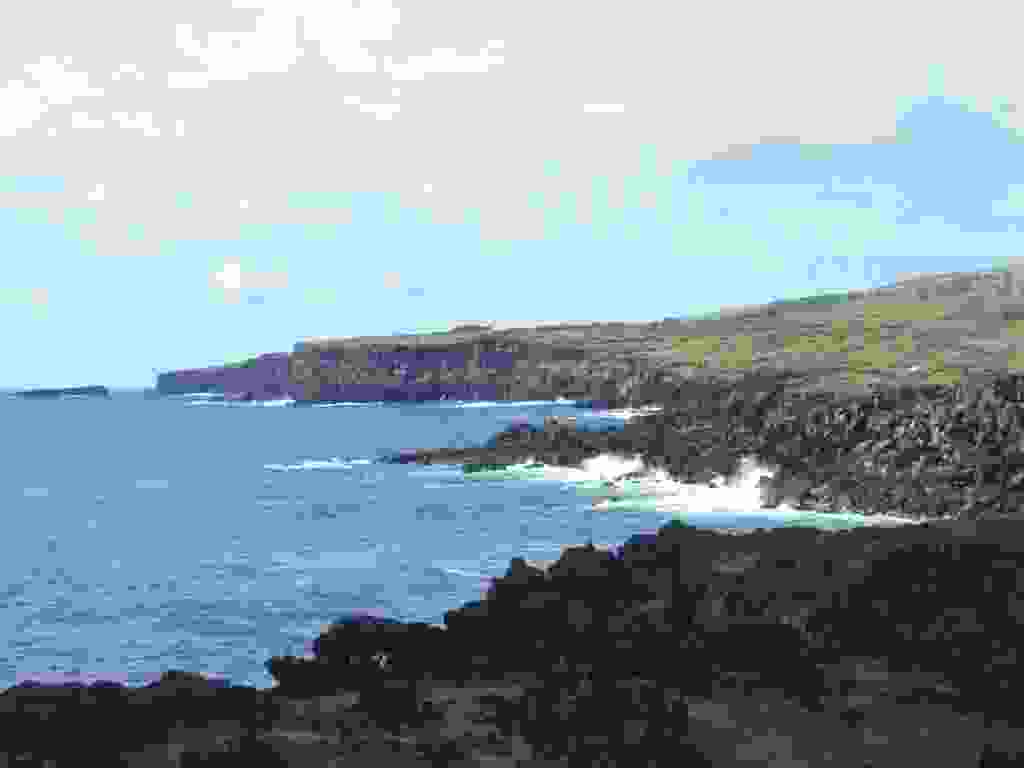
\includegraphics[width=\mywidth]{../wp-content/uploads/2015/03/P3022469-1024x768.jpg} } 
 \newline
 Le lendemain, j´ai loué une voiture avec 2 autres voyageurs rencontrés au camping. \newline
 Départ à 7h pour aller voir le lever du soleil sur les 15 Moais d´Ahu Tongakiri, c'est le site où il y en a le plus debout. \newline
 \newline
\centerline{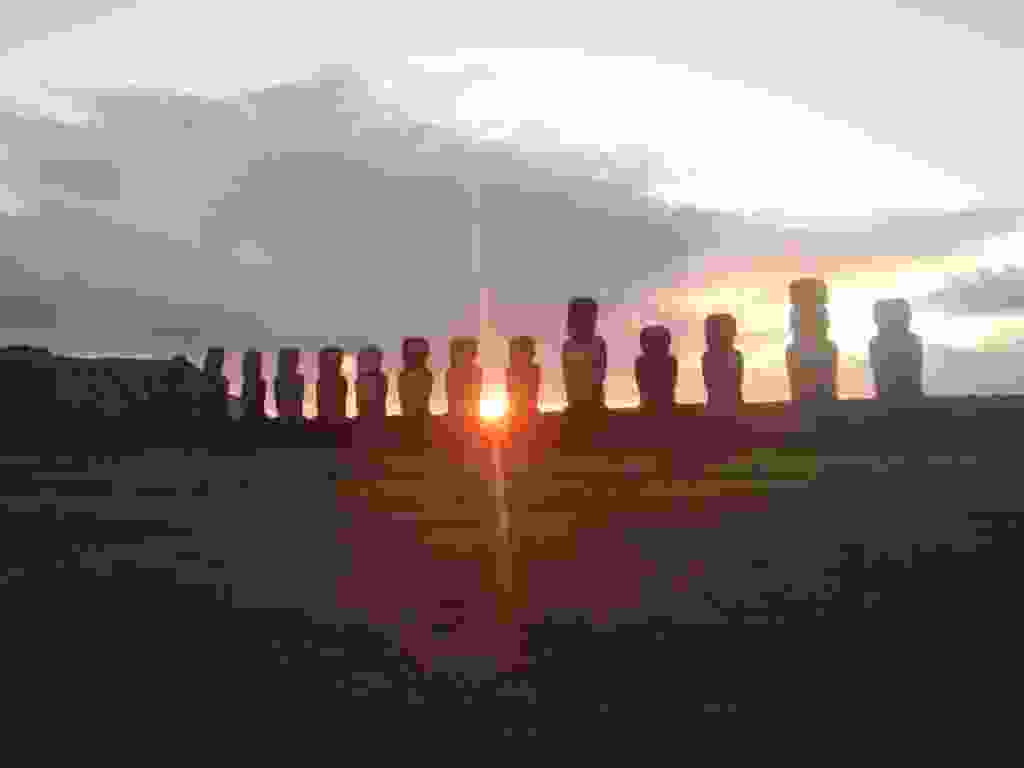
\includegraphics[width=\mywidth]{../wp-content/uploads/2015/03/P3022493-1024x768.jpg} } 
 \newline
\centerline{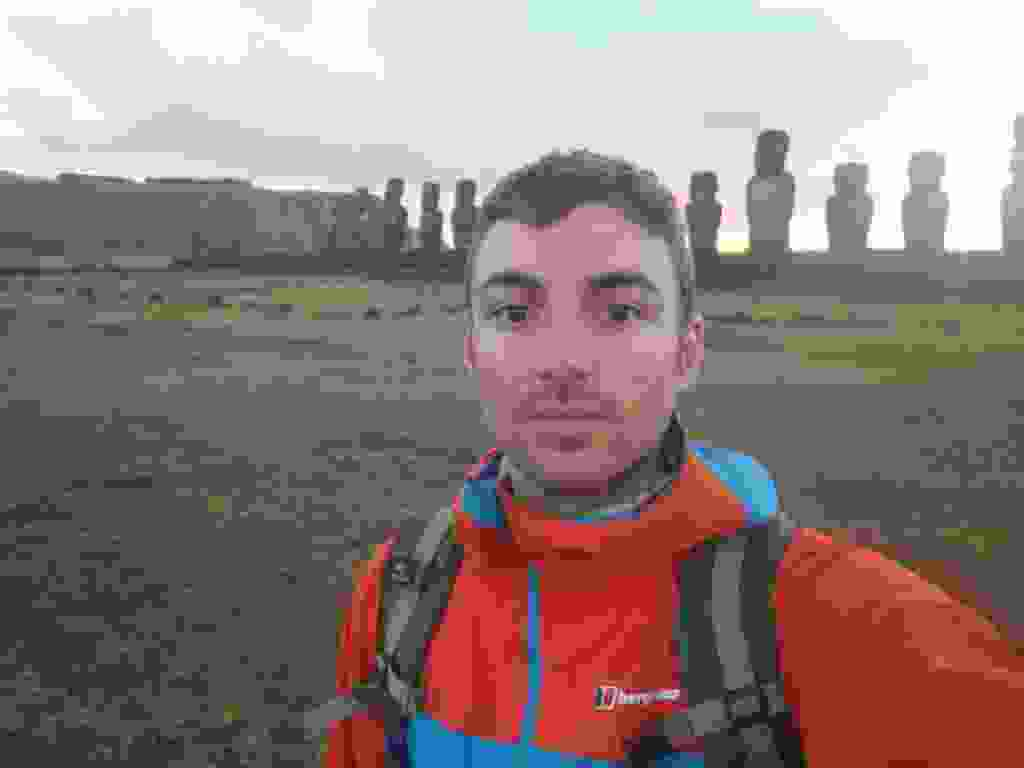
\includegraphics[width=\mywidth]{../wp-content/uploads/2015/03/P3022492-1024x768.jpg} } 
 \newline
 \newline
\centerline{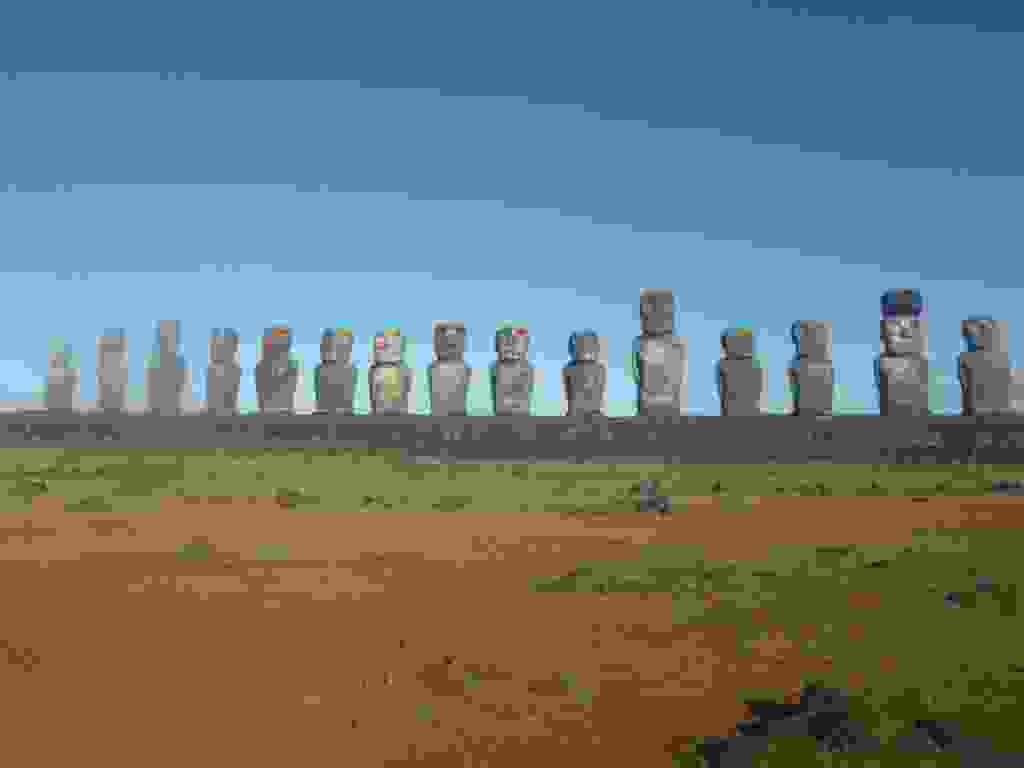
\includegraphics[width=\mywidth]{../wp-content/uploads/2015/03/P3032527-1024x768.jpg} } 
 \newline
\centerline{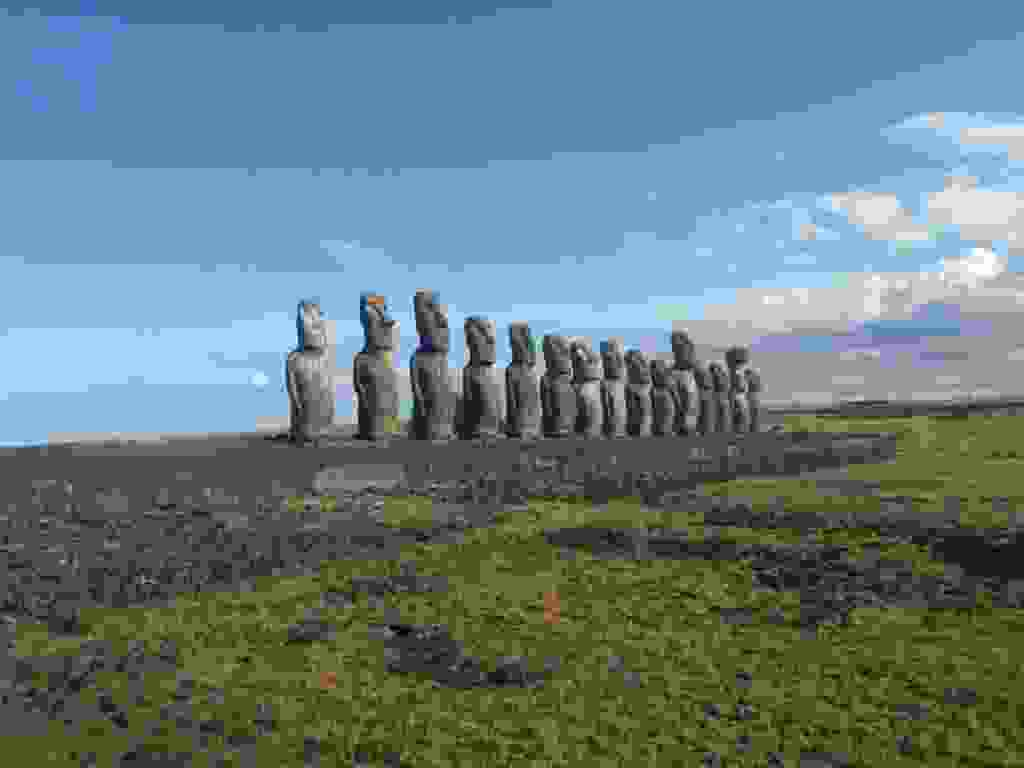
\includegraphics[width=\mywidth]{../wp-content/uploads/2015/03/P3032525-1024x768.jpg} } 
Visite du site de Rano Raraku, là où les moais ont été extraits de la roche, il en reste des dizaines inachevés ou en cours de déplacement. \newline
 \newline
\centerline{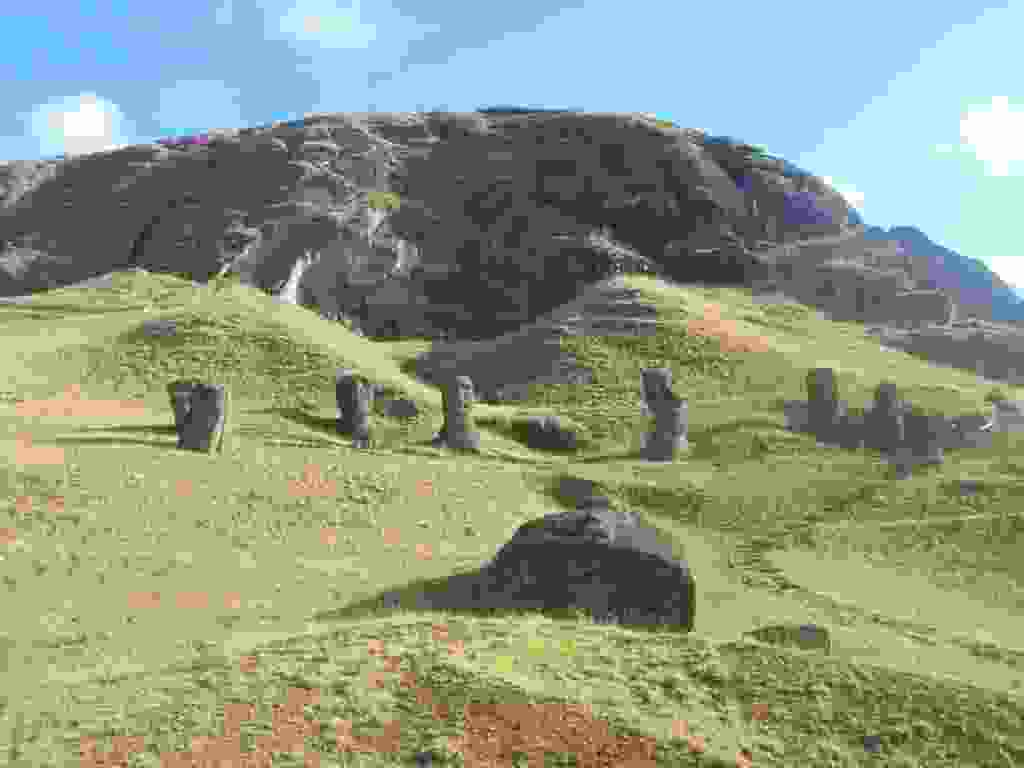
\includegraphics[width=\mywidth]{../wp-content/uploads/2015/03/P3022504-1024x768.jpg} } 
 \newline
\centerline{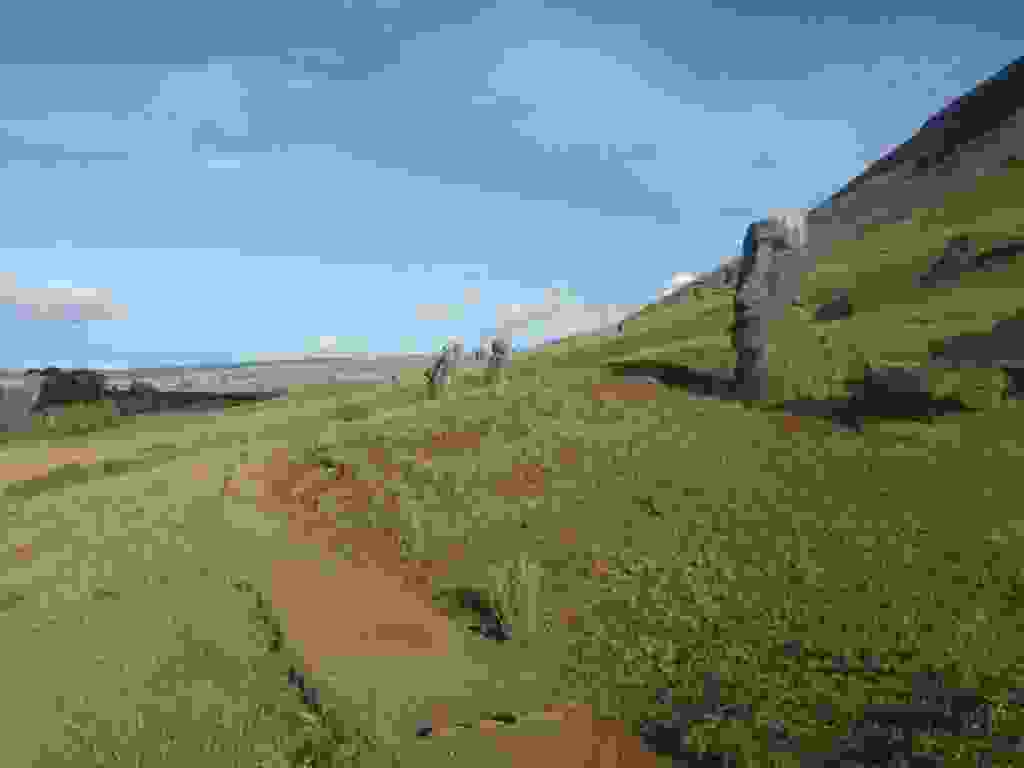
\includegraphics[width=\mywidth]{../wp-content/uploads/2015/03/P3022505-1024x768.jpg} } 
 \newline
 Nous sommes montés au volcan Maunga Terevaka, point culminant de l´île à 511m. \newline
 \newline
\centerline{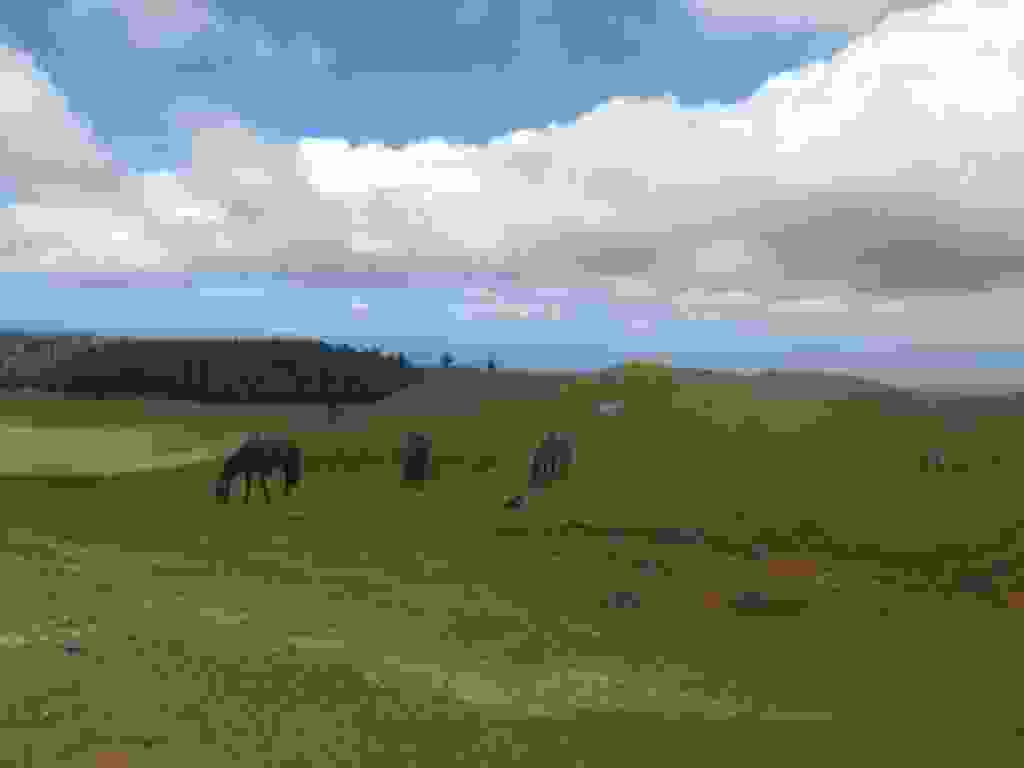
\includegraphics[width=\mywidth]{../wp-content/uploads/2015/03/P3022514-1024x768.jpg} } 
 \newline
 Sandro et Carsten avec qui j´aipartagé la voiture. Sandro voyage depuis 8 ans sans interruption, record à battre !\newline
\centerline{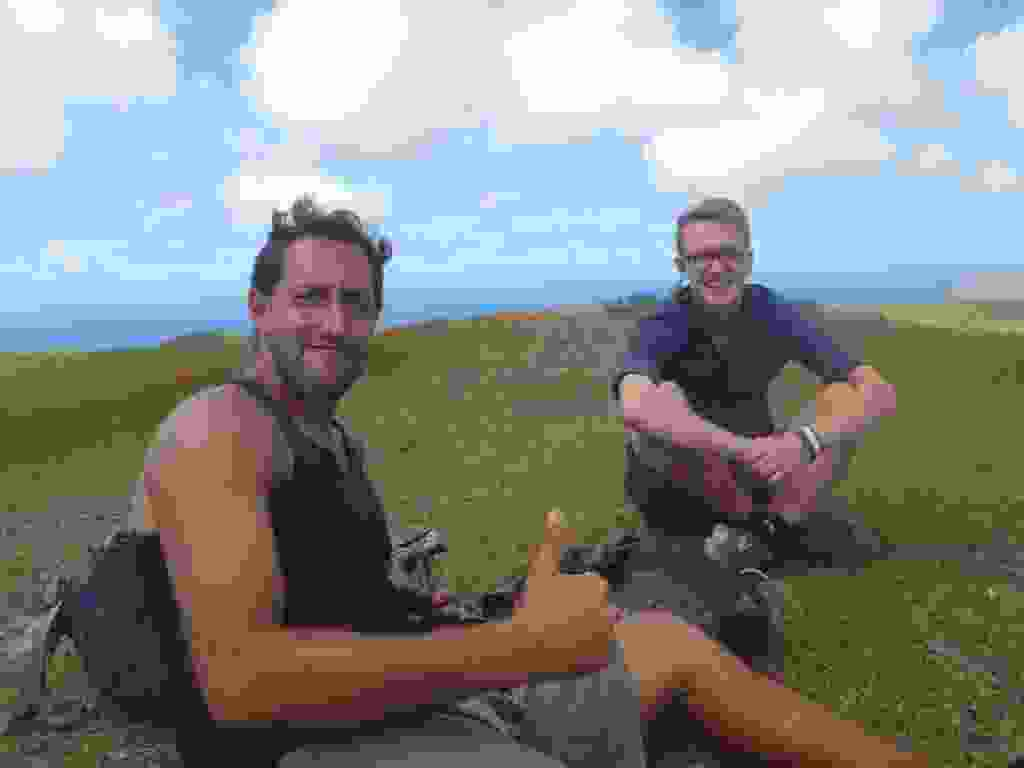
\includegraphics[width=\mywidth]{../wp-content/uploads/2015/03/P3022516-1024x768.jpg} } 
Petit tour à la plage Anakena \newline
 \newline
\centerline{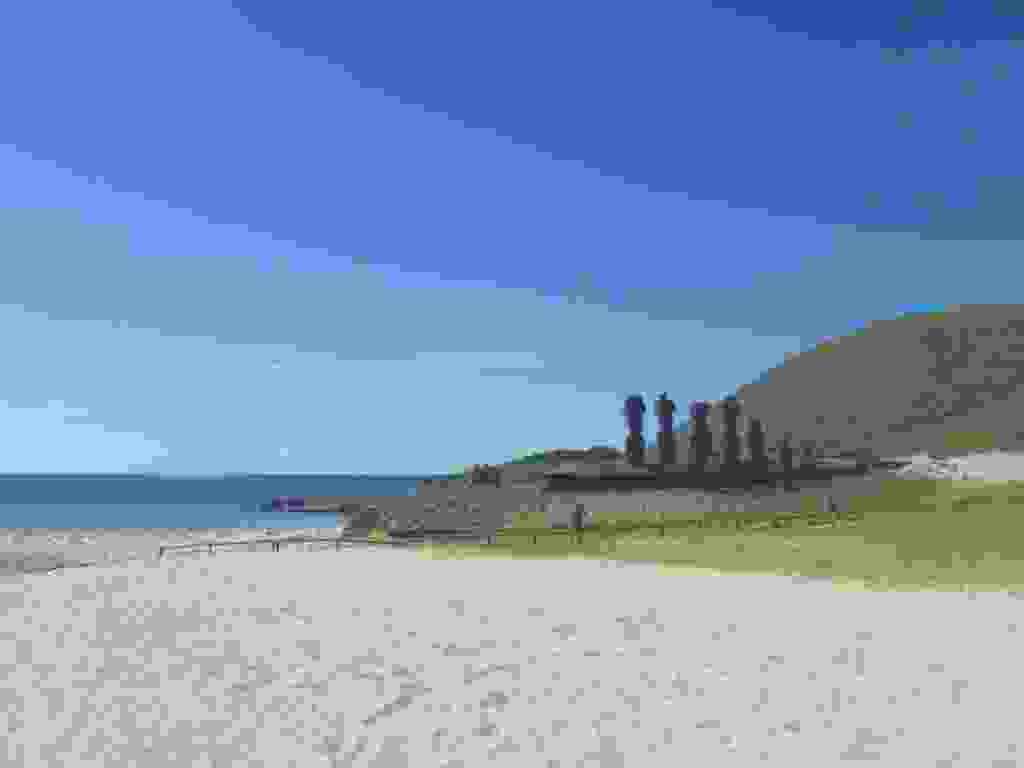
\includegraphics[width=\mywidth]{../wp-content/uploads/2015/03/P3032518-1024x768.jpg} } 
 \newline
\centerline{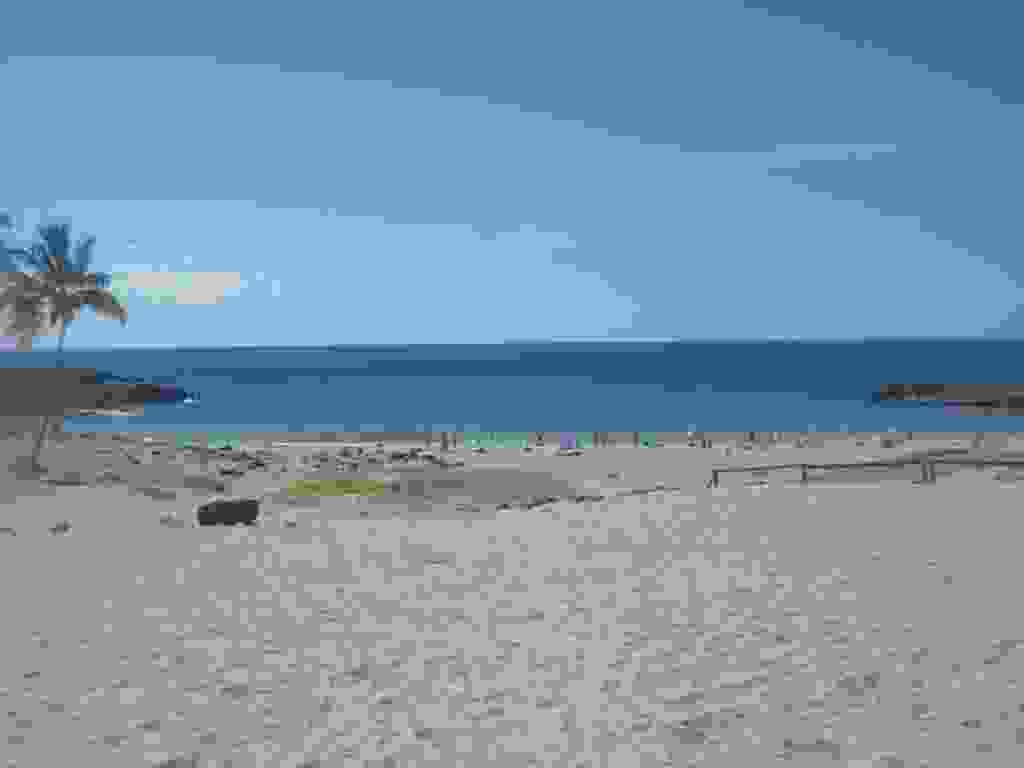
\includegraphics[width=\mywidth]{../wp-content/uploads/2015/03/P3032519-1024x768.jpg} } 
Retour au village pour le coucher du soleil \newline
 \newline
\centerline{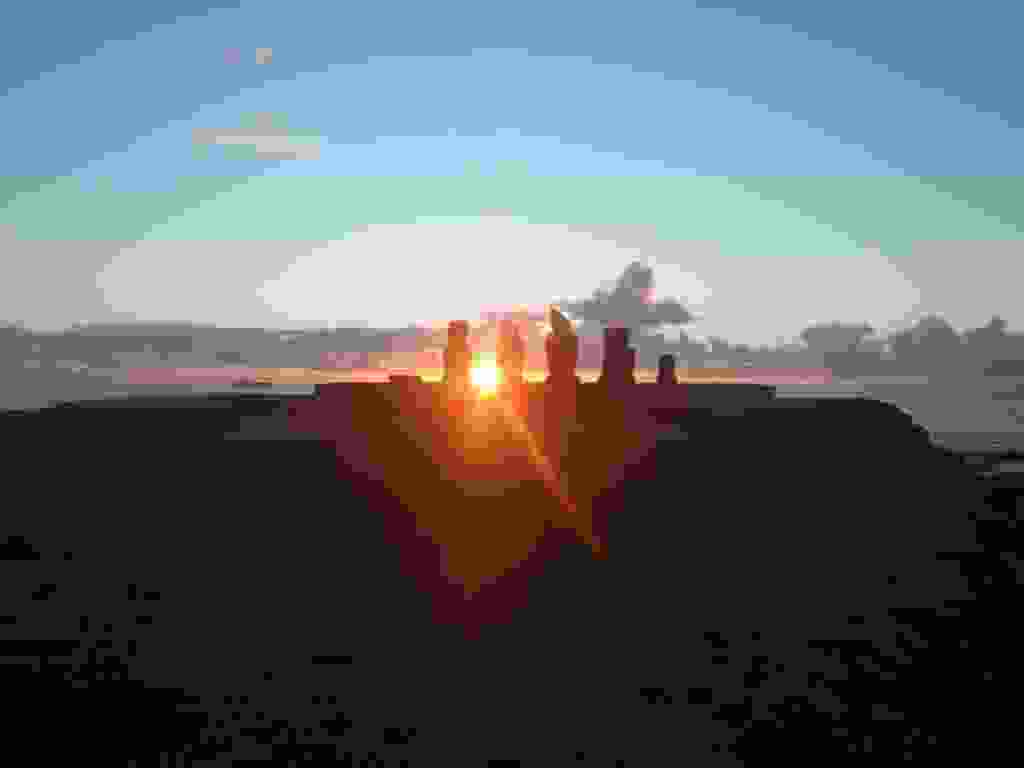
\includegraphics[width=\mywidth]{../wp-content/uploads/2015/03/P3032537-1024x768.jpg} } 
 \newline
\centerline{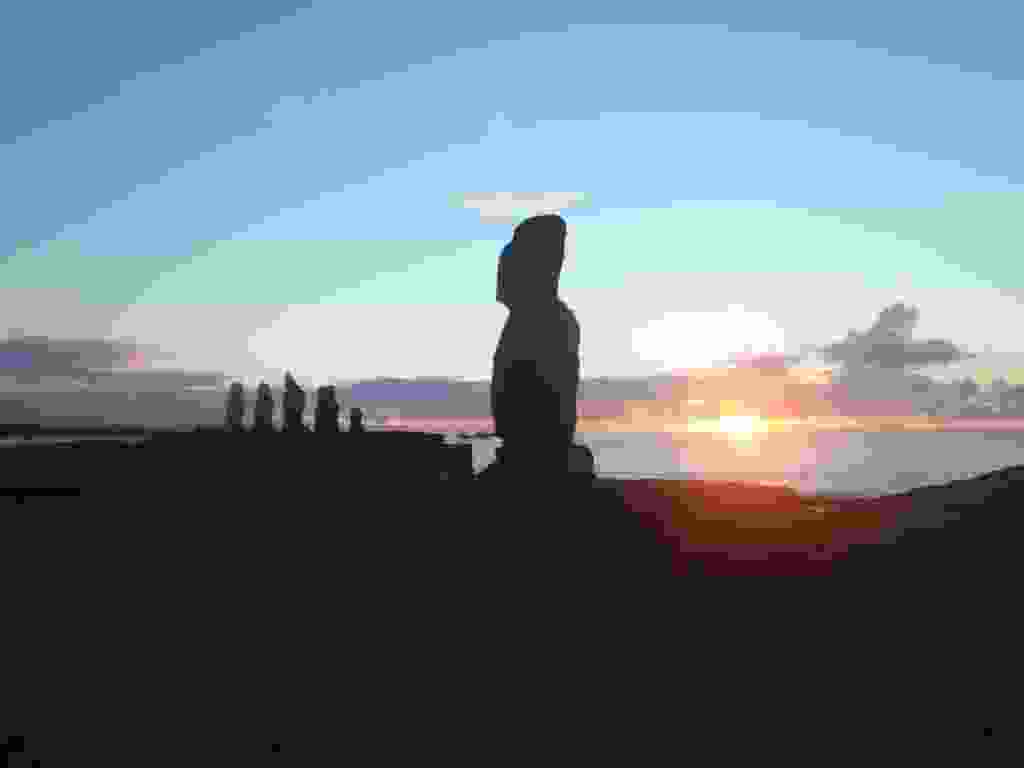
\includegraphics[width=\mywidth]{../wp-content/uploads/2015/03/P3032539-1024x768.jpg} } 
 \newline
 Petite rando le long de la côte, il y a quelques grottes à visiter dont une avec vue sur la mer ! \newline
 \newline
\centerline{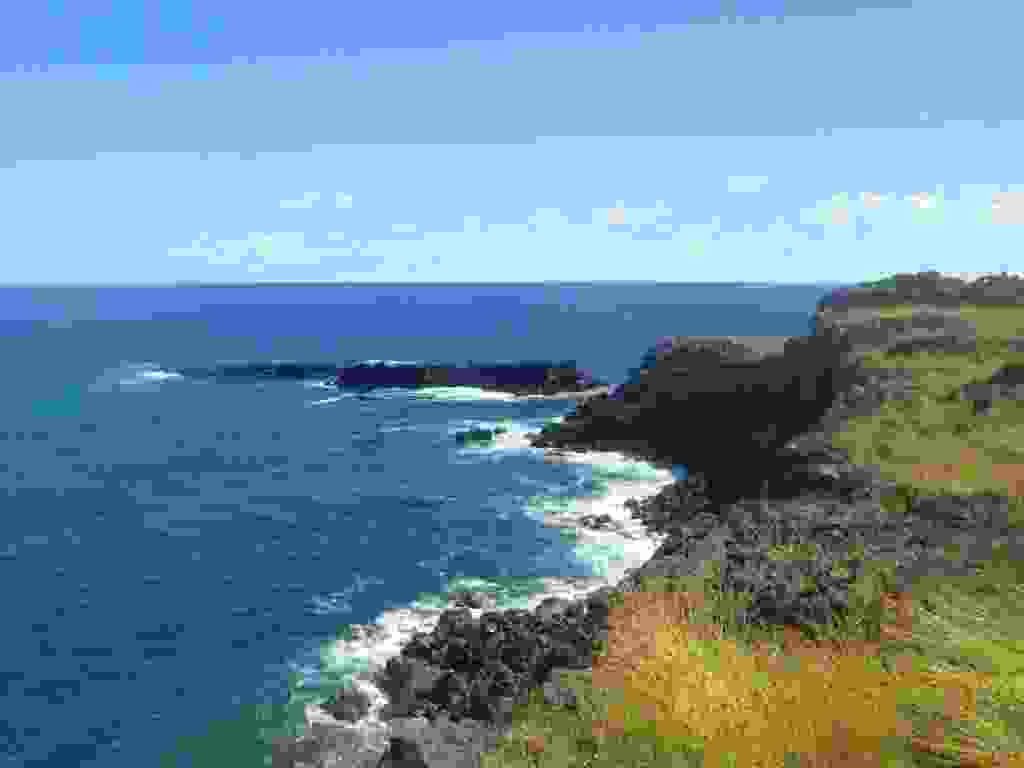
\includegraphics[width=\mywidth]{../wp-content/uploads/2015/03/P3032542-1024x768.jpg} } 
 \newline
\centerline{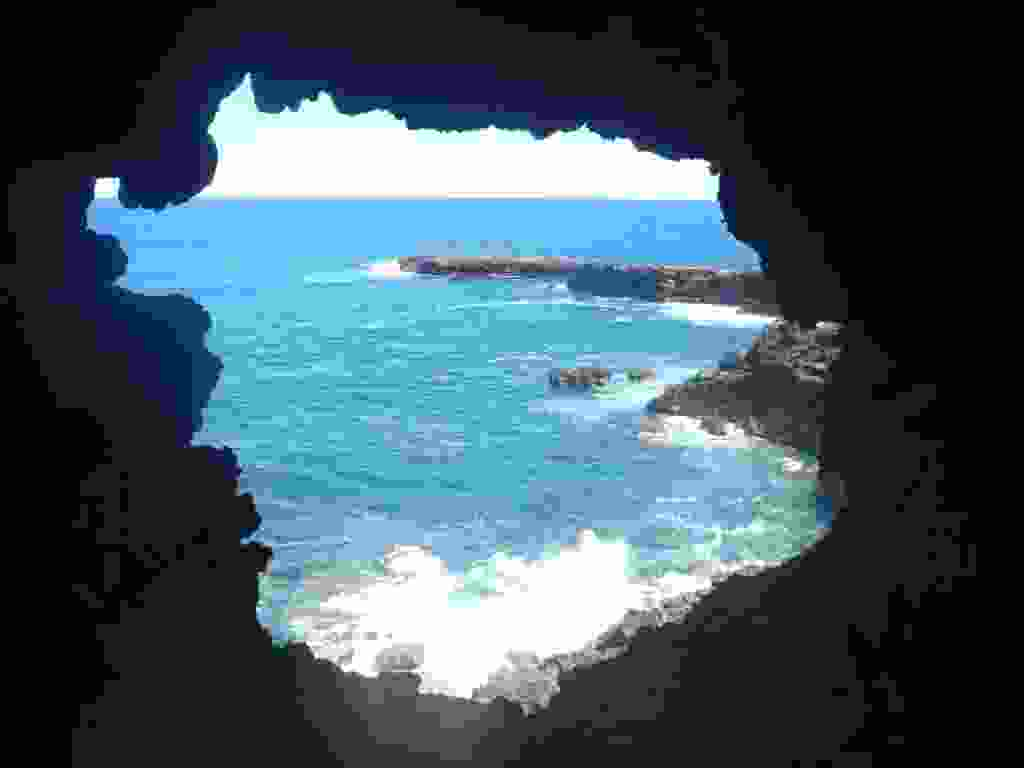
\includegraphics[width=\mywidth]{../wp-content/uploads/2015/03/P3032543-1024x768.jpg} } 
 \newline
 Site d´Orongo, lieu de cérémonie perché entre un cratère et l´océan Pacifique. \newline
 \newline
\centerline{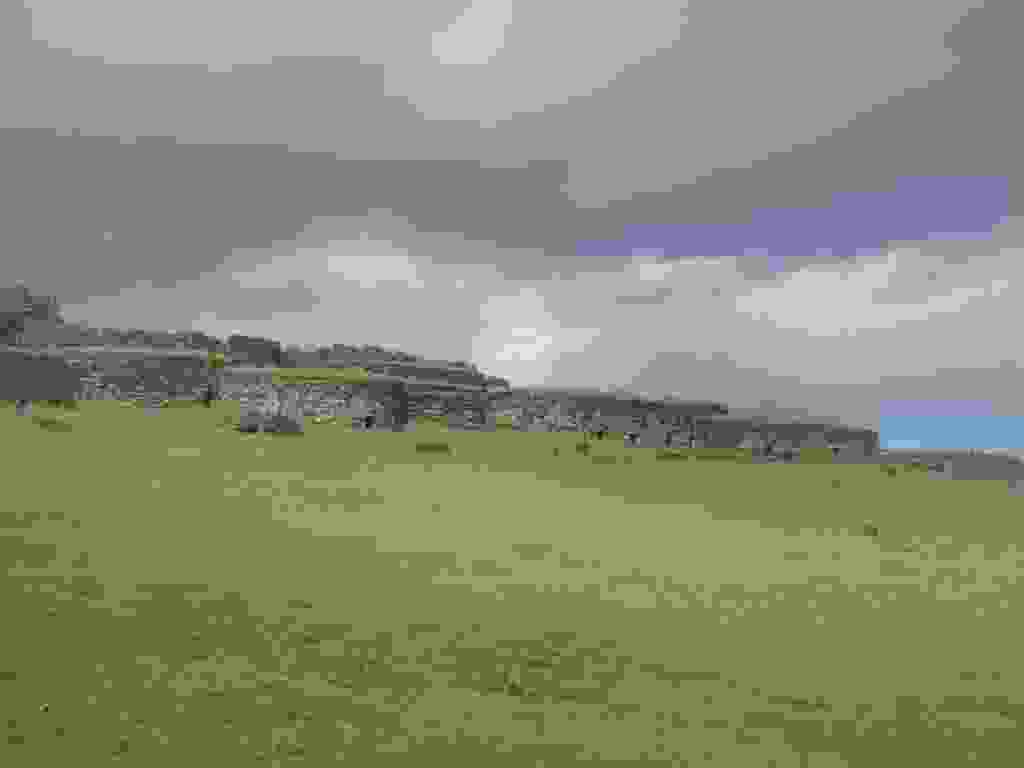
\includegraphics[width=\mywidth]{../wp-content/uploads/2015/03/P3042551-1024x768.jpg} } 
 \newline
\centerline{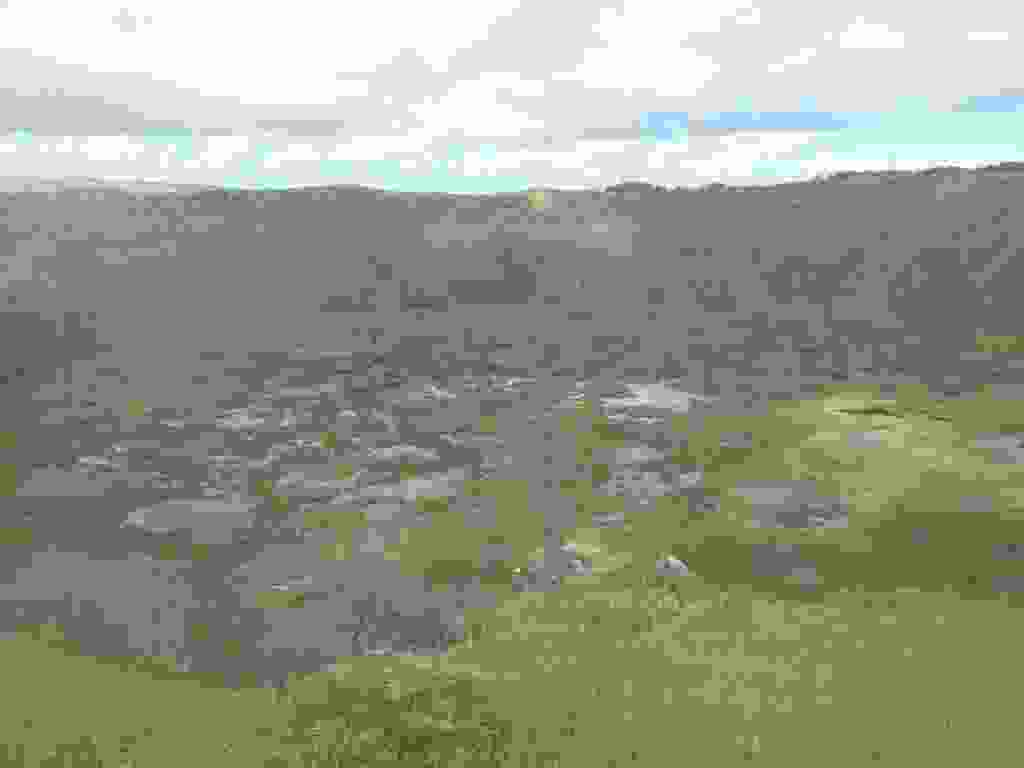
\includegraphics[width=\mywidth]{../wp-content/uploads/2015/03/P3042552-1024x768.jpg} } 
 \newline
 \newline
\centerline{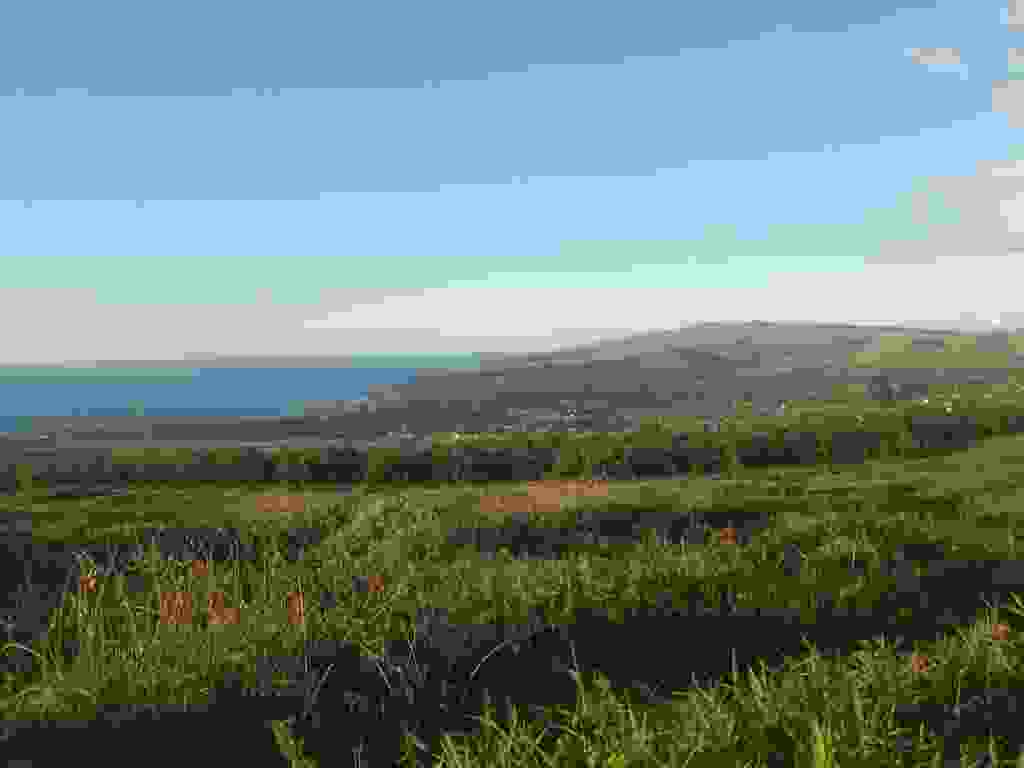
\includegraphics[width=\mywidth]{../wp-content/uploads/2015/03/P3032530-1024x768.jpg} } 
 \newline
\centerline{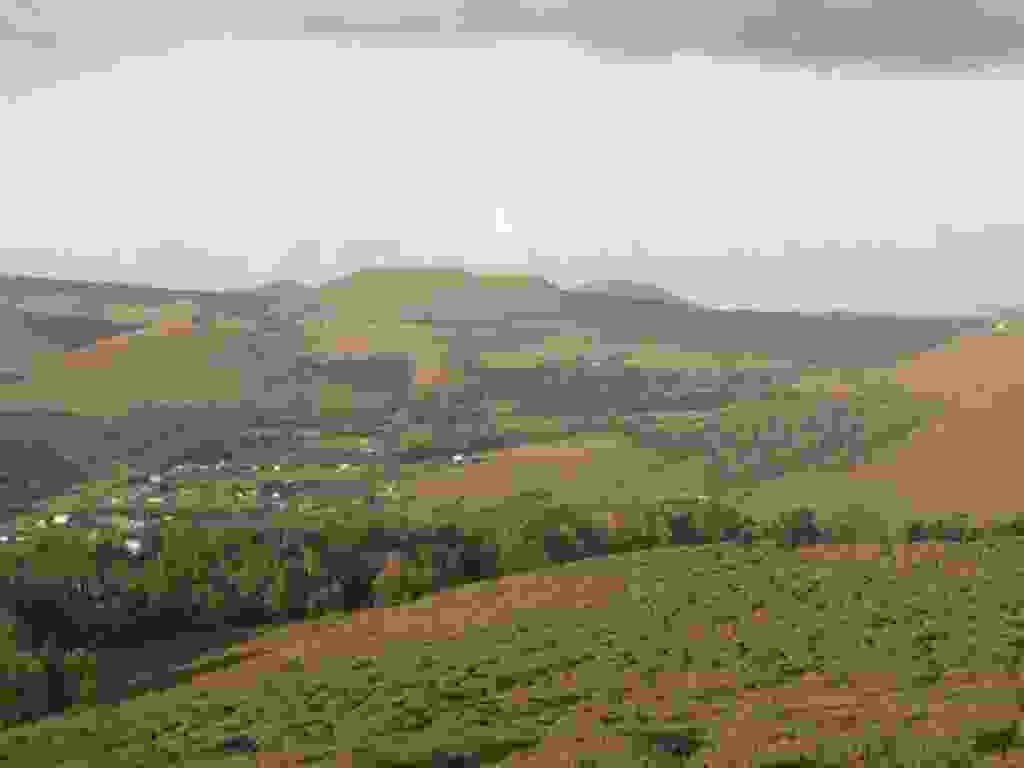
\includegraphics[width=\mywidth]{../wp-content/uploads/2015/03/P3032531-1024x768.jpg} } 
 \newline
  \newline
  \newline
  \newline
  \newline
  \newline
  \newline
  \newline

\newpage
 
